\documentclass{article}\usepackage[]{graphicx}\usepackage[]{color}
%% maxwidth is the original width if it is less than linewidth
%% otherwise use linewidth (to make sure the graphics do not exceed the margin)
\makeatletter
\def\maxwidth{ %
  \ifdim\Gin@nat@width>\linewidth
    \linewidth
  \else
    \Gin@nat@width
  \fi
}
\makeatother

\definecolor{fgcolor}{rgb}{0.345, 0.345, 0.345}
\newcommand{\hlnum}[1]{\textcolor[rgb]{0.686,0.059,0.569}{#1}}%
\newcommand{\hlstr}[1]{\textcolor[rgb]{0.192,0.494,0.8}{#1}}%
\newcommand{\hlcom}[1]{\textcolor[rgb]{0.678,0.584,0.686}{\textit{#1}}}%
\newcommand{\hlopt}[1]{\textcolor[rgb]{0,0,0}{#1}}%
\newcommand{\hlstd}[1]{\textcolor[rgb]{0.345,0.345,0.345}{#1}}%
\newcommand{\hlkwa}[1]{\textcolor[rgb]{0.161,0.373,0.58}{\textbf{#1}}}%
\newcommand{\hlkwb}[1]{\textcolor[rgb]{0.69,0.353,0.396}{#1}}%
\newcommand{\hlkwc}[1]{\textcolor[rgb]{0.333,0.667,0.333}{#1}}%
\newcommand{\hlkwd}[1]{\textcolor[rgb]{0.737,0.353,0.396}{\textbf{#1}}}%

\usepackage{framed}
\makeatletter
\newenvironment{kframe}{%
 \def\at@end@of@kframe{}%
 \ifinner\ifhmode%
  \def\at@end@of@kframe{\end{minipage}}%
  \begin{minipage}{\columnwidth}%
 \fi\fi%
 \def\FrameCommand##1{\hskip\@totalleftmargin \hskip-\fboxsep
 \colorbox{shadecolor}{##1}\hskip-\fboxsep
     % There is no \\@totalrightmargin, so:
     \hskip-\linewidth \hskip-\@totalleftmargin \hskip\columnwidth}%
 \MakeFramed {\advance\hsize-\width
   \@totalleftmargin\z@ \linewidth\hsize
   \@setminipage}}%
 {\par\unskip\endMakeFramed%
 \at@end@of@kframe}
\makeatother

\definecolor{shadecolor}{rgb}{.97, .97, .97}
\definecolor{messagecolor}{rgb}{0, 0, 0}
\definecolor{warningcolor}{rgb}{1, 0, 1}
\definecolor{errorcolor}{rgb}{1, 0, 0}
\newenvironment{knitrout}{}{} % an empty environment to be redefined in TeX

\usepackage{alltt}
\IfFileExists{upquote.sty}{\usepackage{upquote}}{}
\begin{document}

\begin{knitrout}
\definecolor{shadecolor}{rgb}{0.969, 0.969, 0.969}\color{fgcolor}\begin{kframe}
\begin{alltt}
\hlcom{#install.packages("Matching", dependencies=TRUE)}
\hlcom{#install.packages("rgenoud")}
\hlkwd{setwd}\hlstd{(}\hlstr{"C:/Users/Darin/Documents/sanctionsbackslide/Spectrum"}\hlstd{)}
\hlkwd{library}\hlstd{(Matching)}
\hlkwd{library}\hlstd{(rgenoud)}
\hlkwd{library}\hlstd{(dplyr)}
\hlkwd{library}\hlstd{(stargazer)}
\hlkwd{library}\hlstd{(readr)}

\hlstd{df} \hlkwb{<-} \hlkwd{read_csv}\hlstd{(}\hlstr{"SanctionsFinal.csv"}\hlstd{)} \hlopt
  \hlkwd{mutate}\hlstd{(}\hlkwc{pop1} \hlstd{=} \hlkwd{log}\hlstd{(pop1))} \hlopt
  \hlkwd{filter}\hlstd{(}\hlopt{!}\hlkwd{is.na}\hlstd{(GDP_UN))}

\hlstd{df}\hlopt{$}\hlstd{murban[df}\hlopt{$}\hlstd{murban} \hlopt{<} \hlnum{0}\hlstd{]} \hlkwb{<-} \hlnum{0}

\hlstd{dsum} \hlkwb{<-} \hlkwd{as.data.frame}\hlstd{(}\hlkwd{select}\hlstd{(df, polity2, sanctions, GDP_UN, pop1, menergy, mindustry, murban, dpolityb))}

\hlstd{dt} \hlkwb{<-}  \hlstd{df} \hlopt
  \hlkwd{group_by}\hlstd{(sanctions)} \hlopt
  \hlkwd{summarise}\hlstd{(}\hlkwc{polity2} \hlstd{=} \hlkwd{mean}\hlstd{(polity2))}
\hlstd{dt} \hlkwb{<-} \hlkwd{as.data.frame}\hlstd{(dt)}
\end{alltt}
\end{kframe}
\end{knitrout}

\begin{kframe}
\begin{alltt}
\hlkwd{stargazer}\hlstd{(dsum,} \hlkwc{title} \hlstd{=} \hlstr{"Summary Statistics"}\hlstd{)}
\end{alltt}
\end{kframe}
% Table created by stargazer v.5.1 by Marek Hlavac, Harvard University. E-mail: hlavac at fas.harvard.edu
% Date and time: Mon, Nov 02, 2015 - 3:00:08 PM
\begin{table}[!htbp] \centering 
  \caption{Summary Statistics} 
  \label{} 
\begin{tabular}{@{\extracolsep{5pt}}lccccc} 
\\[-1.8ex]\hline 
\hline \\[-1.8ex] 
Statistic & \multicolumn{1}{c}{N} & \multicolumn{1}{c}{Mean} & \multicolumn{1}{c}{St. Dev.} & \multicolumn{1}{c}{Min} & \multicolumn{1}{c}{Max} \\ 
\hline \\[-1.8ex] 
polity2 & 4,043 & 0.153 & 7.555 & $-$10 & 10 \\ 
sanctions & 4,043 & 0.197 & 0.398 & 0 & 1 \\ 
GDP\_UN & 4,043 & 3,902.012 & 6,605.237 & 14 & 43,165 \\ 
pop1 & 4,043 & 8.987 & 1.544 & 4.984 & 14.065 \\ 
menergy & 4,043 & 5.621 & 1.954 & 0.000 & 12.261 \\ 
mindustry & 4,043 & 37.808 & 10.452 & 2.000 & 85.000 \\ 
murban & 4,043 & 8,735.562 & 30,395.150 & 0.000 & 531,307.000 \\ 
dpolityb & 4,008 & 0.109 & 0.312 & 0 & 1 \\ 
\hline \\[-1.8ex] 
\end{tabular} 
\end{table} 
\begin{kframe}\begin{alltt}
\hlkwd{stargazer}\hlstd{(dt,} \hlkwc{summary} \hlstd{= F,} \hlkwc{title} \hlstd{=} \hlstr{"Average Score of Democracy: Sanctioned vs Non-Sanctioned"}\hlstd{,} \hlkwc{rownames} \hlstd{= F)}
\end{alltt}
\end{kframe}
% Table created by stargazer v.5.1 by Marek Hlavac, Harvard University. E-mail: hlavac at fas.harvard.edu
% Date and time: Mon, Nov 02, 2015 - 3:00:08 PM
\begin{table}[!htbp] \centering 
  \caption{Average Score of Democracy: Sanctioned vs Non-Sanctioned} 
  \label{} 
\begin{tabular}{@{\extracolsep{5pt}} cc} 
\\[-1.8ex]\hline 
\hline \\[-1.8ex] 
sanctions & polity2 \\ 
\hline \\[-1.8ex] 
$0$ & $0.518$ \\ 
$1$ & $$-$1.332$ \\ 
\hline \\[-1.8ex] 
\end{tabular} 
\end{table} 


\begin{knitrout}
\definecolor{shadecolor}{rgb}{0.969, 0.969, 0.969}\color{fgcolor}\begin{kframe}
\begin{alltt}
\hlstd{X} \hlkwb{<-} \hlkwd{select}\hlstd{(df, GDP_UN, pop1, menergy, mindustry, murban)}

\hlstd{BalanceMatrix} \hlkwb{<-} \hlkwd{cbind}\hlstd{(df}\hlopt{$}\hlstd{GDP_UN, df}\hlopt{$}\hlstd{pop1, df}\hlopt{$}\hlstd{menergy, df}\hlopt{$}\hlstd{mindustry, df}\hlopt{$}\hlstd{murban,} \hlkwd{I}\hlstd{(df}\hlopt{$}\hlstd{GDP_UN}\hlopt{*}\hlstd{df}\hlopt{$}\hlstd{pop1),} \hlkwd{I}\hlstd{(df}\hlopt{$}\hlstd{GDP_UN}\hlopt{*}\hlstd{df}\hlopt{$}\hlstd{menergy),}
                        \hlkwd{I}\hlstd{(df}\hlopt{$}\hlstd{GDP_UN}\hlopt{*}\hlstd{df}\hlopt{$}\hlstd{mindustry),} \hlkwd{I}\hlstd{(df}\hlopt{$}\hlstd{GDP_UN}\hlopt{*}\hlstd{df}\hlopt{$}\hlstd{murban),} \hlkwd{I}\hlstd{(df}\hlopt{$}\hlstd{pop1}\hlopt{*}\hlstd{df}\hlopt{$}\hlstd{murban),} \hlkwd{I}\hlstd{(df}\hlopt{$}\hlstd{murban}\hlopt{*}\hlstd{df}\hlopt{$}\hlstd{mindustry),}\hlkwd{I}\hlstd{(df}\hlopt{$}\hlstd{pop1}\hlopt{*}\hlstd{df}\hlopt{$}\hlstd{mindustry))}

\hlstd{gen1} \hlkwb{<-} \hlkwd{GenMatch}\hlstd{(}\hlkwc{Tr} \hlstd{= df}\hlopt{$}\hlstd{sanctions,} \hlkwc{X} \hlstd{= X,} \hlkwc{BalanceMatrix} \hlstd{= BalanceMatrix,} \hlkwc{pop.size} \hlstd{=} \hlnum{10}\hlstd{)}
\end{alltt}
\begin{verbatim}
## 
## 
## Mon Nov 02 15:00:09 2015
## Domains:
##  0.000000e+00   <=  X1   <=    1.000000e+03 
##  0.000000e+00   <=  X2   <=    1.000000e+03 
##  0.000000e+00   <=  X3   <=    1.000000e+03 
##  0.000000e+00   <=  X4   <=    1.000000e+03 
##  0.000000e+00   <=  X5   <=    1.000000e+03 
## 
## Data Type: Floating Point
## Operators (code number, name, population) 
## 	(1) Cloning........................... 	0
## 	(2) Uniform Mutation.................. 	1
## 	(3) Boundary Mutation................. 	1
## 	(4) Non-Uniform Mutation.............. 	1
## 	(5) Polytope Crossover................ 	1
## 	(6) Simple Crossover.................. 	2
## 	(7) Whole Non-Uniform Mutation........ 	1
## 	(8) Heuristic Crossover............... 	2
## 	(9) Local-Minimum Crossover........... 	0
## 
## SOFT Maximum Number of Generations: 100
## Maximum Nonchanging Generations: 4
## Population size       : 10
## Convergence Tolerance: 1.000000e-03
## 
## Not Using the BFGS Derivative Based Optimizer on the Best Individual Each Generation.
## Not Checking Gradients before Stopping.
## Using Out of Bounds Individuals.
## 
## Maximization Problem.
## GENERATION: 0 (initializing the population)
## Lexical Fit..... 4.714527e-04  2.299518e-03  3.147996e-03  3.582045e-03  9.971920e-03  1.876782e-02  1.997751e-02  2.055215e-02  3.910067e-02  6.032230e-02  9.801513e-02  9.832089e-02  1.506106e-01  1.761100e-01  2.516666e-01  2.593899e-01  2.956880e-01  3.043066e-01  3.568916e-01  3.904017e-01  5.723546e-01  6.247935e-01  6.247935e-01  7.901177e-01  
## #unique......... 10, #Total UniqueCount: 10
## var 1:
## best............ 1.927923e+02
## mean............ 4.669902e+02
## variance........ 1.175986e+05
## var 2:
## best............ 6.908474e+02
## mean............ 4.813716e+02
## variance........ 1.173796e+05
## var 3:
## best............ 1.653877e+02
## mean............ 5.677351e+02
## variance........ 1.112741e+05
## var 4:
## best............ 2.184367e+01
## mean............ 4.405547e+02
## variance........ 1.320683e+05
## var 5:
## best............ 5.950875e+02
## mean............ 4.063405e+02
## variance........ 1.120444e+05
## 
## GENERATION: 1
## Lexical Fit..... 9.678060e-04  2.168151e-03  5.089865e-03  7.056201e-03  7.117076e-03  8.460487e-03  9.483788e-03  9.971920e-03  2.536250e-02  2.536250e-02  4.949872e-02  5.153005e-02  5.893353e-02  7.513065e-02  1.019353e-01  1.250876e-01  1.533092e-01  1.560254e-01  1.985480e-01  3.270113e-01  3.436753e-01  5.416970e-01  9.773120e-01  9.971154e-01  
## #unique......... 9, #Total UniqueCount: 19
## var 1:
## best............ 5.068376e+01
## mean............ 1.999897e+02
## variance........ 1.040164e+04
## var 2:
## best............ 7.719775e+02
## mean............ 6.542473e+02
## variance........ 2.761785e+04
## var 3:
## best............ 1.195896e+02
## mean............ 3.118353e+02
## variance........ 5.574966e+04
## var 4:
## best............ 9.509240e+02
## mean............ 3.198305e+02
## variance........ 1.465488e+05
## var 5:
## best............ 9.587737e+02
## mean............ 8.138168e+02
## variance........ 2.977944e+04
## 
## GENERATION: 2
## Lexical Fit..... 1.424364e-03  2.854093e-03  6.044482e-03  7.268840e-03  9.971920e-03  1.374916e-02  2.162649e-02  2.184479e-02  2.305650e-02  2.937286e-02  5.153005e-02  5.893353e-02  6.564731e-02  7.538896e-02  9.330430e-02  1.394735e-01  1.405550e-01  1.555043e-01  3.089098e-01  3.151396e-01  4.867242e-01  5.016090e-01  9.773120e-01  9.971154e-01  
## #unique......... 7, #Total UniqueCount: 26
## var 1:
## best............ 4.608889e+01
## mean............ 7.758797e+01
## variance........ 2.949482e+03
## var 2:
## best............ 7.746007e+02
## mean............ 7.098544e+02
## variance........ 1.835571e+04
## var 3:
## best............ 1.181088e+02
## mean............ 1.906628e+02
## variance........ 1.238775e+04
## var 4:
## best............ 9.809645e+02
## mean............ 7.724594e+02
## variance........ 1.191711e+05
## var 5:
## best............ 9.705330e+02
## mean............ 8.542124e+02
## variance........ 2.369435e+04
## 
## GENERATION: 3
## Lexical Fit..... 1.424364e-03  2.854093e-03  6.044482e-03  7.268840e-03  9.971920e-03  1.374916e-02  2.162649e-02  2.184479e-02  2.305650e-02  2.937286e-02  5.153005e-02  5.893353e-02  6.564731e-02  7.538896e-02  9.330430e-02  1.394735e-01  1.405550e-01  1.555043e-01  3.089098e-01  3.151396e-01  4.867242e-01  5.016090e-01  9.773120e-01  9.971154e-01  
## #unique......... 7, #Total UniqueCount: 33
## var 1:
## best............ 4.608889e+01
## mean............ 1.057613e+02
## variance........ 1.883227e+04
## var 2:
## best............ 7.746007e+02
## mean............ 7.545992e+02
## variance........ 7.619782e+03
## var 3:
## best............ 1.181088e+02
## mean............ 1.417075e+02
## variance........ 1.445524e+04
## var 4:
## best............ 9.809645e+02
## mean............ 9.582721e+02
## variance........ 1.800560e+03
## var 5:
## best............ 9.705330e+02
## mean............ 9.611305e+02
## variance........ 3.557963e+02
## 
## GENERATION: 4
## Lexical Fit..... 1.424364e-03  2.854093e-03  6.044482e-03  7.268840e-03  9.971920e-03  1.374916e-02  2.162649e-02  2.184479e-02  2.305650e-02  2.937286e-02  5.153005e-02  5.893353e-02  6.564731e-02  7.538896e-02  9.330430e-02  1.394735e-01  1.405550e-01  1.555043e-01  3.089098e-01  3.151396e-01  4.867242e-01  5.016090e-01  9.773120e-01  9.971154e-01  
## #unique......... 8, #Total UniqueCount: 41
## var 1:
## best............ 4.608889e+01
## mean............ 5.868395e+01
## variance........ 2.078953e+03
## var 2:
## best............ 7.746007e+02
## mean............ 7.735409e+02
## variance........ 1.066289e+01
## var 3:
## best............ 1.181088e+02
## mean............ 1.775666e+02
## variance........ 3.198792e+04
## var 4:
## best............ 9.809645e+02
## mean............ 9.215829e+02
## variance........ 1.478850e+04
## var 5:
## best............ 9.705330e+02
## mean............ 9.364306e+02
## variance........ 4.950395e+03
## 
## GENERATION: 5
## Lexical Fit..... 1.424364e-03  2.854093e-03  6.044482e-03  7.268840e-03  9.971920e-03  1.374916e-02  2.162649e-02  2.184479e-02  2.305650e-02  2.937286e-02  5.153005e-02  5.893353e-02  6.564731e-02  7.538896e-02  9.330430e-02  1.394735e-01  1.405550e-01  1.555043e-01  3.089098e-01  3.151396e-01  4.867242e-01  5.016090e-01  9.773120e-01  9.971154e-01  
## #unique......... 5, #Total UniqueCount: 46
## var 1:
## best............ 4.608889e+01
## mean............ 4.826822e+01
## variance........ 5.156063e+01
## var 2:
## best............ 7.746007e+02
## mean............ 7.319363e+02
## variance........ 1.621537e+04
## var 3:
## best............ 1.181088e+02
## mean............ 1.185059e+02
## variance........ 2.051905e+00
## var 4:
## best............ 9.809645e+02
## mean............ 9.182221e+02
## variance........ 1.748334e+04
## var 5:
## best............ 9.705330e+02
## mean............ 9.287696e+02
## variance........ 1.648753e+04
## 
## GENERATION: 6
## Lexical Fit..... 1.424364e-03  2.854093e-03  6.044482e-03  7.268840e-03  9.971920e-03  1.374916e-02  2.162649e-02  2.184479e-02  2.305650e-02  2.937286e-02  5.153005e-02  5.893353e-02  6.564731e-02  7.538896e-02  9.330430e-02  1.394735e-01  1.405550e-01  1.555043e-01  3.089098e-01  3.151396e-01  4.867242e-01  5.016090e-01  9.773120e-01  9.971154e-01  
## #unique......... 8, #Total UniqueCount: 54
## var 1:
## best............ 4.608889e+01
## mean............ 1.071087e+02
## variance........ 2.551809e+04
## var 2:
## best............ 7.746007e+02
## mean............ 7.772103e+02
## variance........ 7.286933e+03
## var 3:
## best............ 1.181088e+02
## mean............ 1.175622e+02
## variance........ 2.107664e+02
## var 4:
## best............ 9.809645e+02
## mean............ 9.270602e+02
## variance........ 1.277711e+04
## var 5:
## best............ 9.705330e+02
## mean............ 9.720136e+02
## variance........ 9.212002e+00
## 
## GENERATION: 7
## Lexical Fit..... 1.424364e-03  2.854093e-03  6.044482e-03  7.268840e-03  9.971920e-03  1.374916e-02  2.162649e-02  2.184479e-02  2.305650e-02  2.937286e-02  5.153005e-02  5.893353e-02  6.564731e-02  7.538896e-02  9.330430e-02  1.394735e-01  1.405550e-01  1.555043e-01  3.089098e-01  3.151396e-01  4.867242e-01  5.016090e-01  9.773120e-01  9.971154e-01  
## #unique......... 8, #Total UniqueCount: 62
## var 1:
## best............ 4.608889e+01
## mean............ 7.768395e+01
## variance........ 9.591236e+03
## var 2:
## best............ 7.746007e+02
## mean............ 7.740022e+02
## variance........ 3.804271e+00
## var 3:
## best............ 1.181088e+02
## mean............ 1.723867e+02
## variance........ 2.693666e+04
## var 4:
## best............ 9.809645e+02
## mean............ 9.378040e+02
## variance........ 1.722392e+04
## var 5:
## best............ 9.705330e+02
## mean............ 9.574201e+02
## variance........ 1.602157e+03
## 
## 'wait.generations' limit reached.
## No significant improvement in 4 generations.
## 
## Solution Lexical Fitness Value:
## 1.424364e-03  2.854093e-03  6.044482e-03  7.268840e-03  9.971920e-03  1.374916e-02  2.162649e-02  2.184479e-02  2.305650e-02  2.937286e-02  5.153005e-02  5.893353e-02  6.564731e-02  7.538896e-02  9.330430e-02  1.394735e-01  1.405550e-01  1.555043e-01  3.089098e-01  3.151396e-01  4.867242e-01  5.016090e-01  9.773120e-01  9.971154e-01  
## 
## Parameters at the Solution:
## 
##  X[ 1] :	4.608889e+01
##  X[ 2] :	7.746007e+02
##  X[ 3] :	1.181088e+02
##  X[ 4] :	9.809645e+02
##  X[ 5] :	9.705330e+02
## 
## Solution Found Generation 2
## Number of Generations Run 7
## 
## Mon Nov 02 15:00:37 2015
## Total run time : 0 hours 0 minutes and 28 seconds
\end{verbatim}
\begin{alltt}
\hlstd{mgen1} \hlkwb{<-} \hlkwd{Match}\hlstd{(}\hlkwc{Y} \hlstd{= df}\hlopt{$}\hlstd{polity2,} \hlkwc{Tr} \hlstd{= df}\hlopt{$}\hlstd{sanctions,} \hlkwc{X} \hlstd{= X,} \hlkwc{Weight.matrix} \hlstd{= gen1)}
\hlkwd{print}\hlstd{(}\hlkwd{summary}\hlstd{(mgen1))}
\end{alltt}
\begin{verbatim}
## 
## Estimate...  -0.96738 
## AI SE......  0.34803 
## T-stat.....  -2.7795 
## p.val......  0.0054434 
## 
## Original number of observations..............  4043 
## Original number of treated obs...............  797 
## Matched number of observations...............  797 
## Matched number of observations  (unweighted).  797
\end{verbatim}
\end{kframe}
\end{knitrout}

\begin{knitrout}
\definecolor{shadecolor}{rgb}{0.969, 0.969, 0.969}\color{fgcolor}\begin{kframe}
\begin{alltt}
\hlkwd{qqplot}\hlstd{(df}\hlopt{$}\hlstd{GDP_UN[mgen1}\hlopt{$}\hlstd{index.treated], df}\hlopt{$}\hlstd{GDP_UN[mgen1}\hlopt{$}\hlstd{index.control],}
                 \hlkwc{xlab} \hlstd{=} \hlstr{"Treated"}\hlstd{,} \hlkwc{ylab} \hlstd{=} \hlstr{"Control"}\hlstd{,} \hlkwc{main} \hlstd{=} \hlstr{"QQ Plot of Distribution of GDP"}\hlstd{)}
\end{alltt}
\end{kframe}
\includegraphics[width=\maxwidth]{figure/unnamed-chunk-3-1} 
\begin{kframe}\begin{alltt}
\hlkwd{qqplot}\hlstd{(df}\hlopt{$}\hlstd{pop1[mgen1}\hlopt{$}\hlstd{index.treated], df}\hlopt{$}\hlstd{pop1[mgen1}\hlopt{$}\hlstd{index.control],}
                 \hlkwc{xlab} \hlstd{=} \hlstr{"Treated"}\hlstd{,} \hlkwc{ylab} \hlstd{=} \hlstr{"Control"}\hlstd{,} \hlkwc{main} \hlstd{=} \hlstr{"QQ Plot of Distribution of GDP"}\hlstd{)}
\end{alltt}
\end{kframe}
\includegraphics[width=\maxwidth]{figure/unnamed-chunk-3-2} 
\begin{kframe}\begin{alltt}
\hlkwd{qqplot}\hlstd{(df}\hlopt{$}\hlstd{menergy[mgen1}\hlopt{$}\hlstd{index.treated], df}\hlopt{$}\hlstd{menergy[mgen1}\hlopt{$}\hlstd{index.control],}
                 \hlkwc{xlab} \hlstd{=} \hlstr{"Treated"}\hlstd{,} \hlkwc{ylab} \hlstd{=} \hlstr{"Control"}\hlstd{,} \hlkwc{main} \hlstd{=} \hlstr{"QQ Plot of Distribution of GDP"}\hlstd{)}
\end{alltt}
\end{kframe}
\includegraphics[width=\maxwidth]{figure/unnamed-chunk-3-3} 
\begin{kframe}\begin{alltt}
\hlkwd{qqplot}\hlstd{(df}\hlopt{$}\hlstd{mindustry[mgen1}\hlopt{$}\hlstd{index.treated], df}\hlopt{$}\hlstd{mindustry[mgen1}\hlopt{$}\hlstd{index.control],}
                 \hlkwc{xlab} \hlstd{=} \hlstr{"Treated"}\hlstd{,} \hlkwc{ylab} \hlstd{=} \hlstr{"Control"}\hlstd{,} \hlkwc{main} \hlstd{=} \hlstr{"QQ Plot of Distribution of GDP"}\hlstd{)}
\end{alltt}
\end{kframe}
\includegraphics[width=\maxwidth]{figure/unnamed-chunk-3-4} 
\begin{kframe}\begin{alltt}
\hlkwd{qqplot}\hlstd{(df}\hlopt{$}\hlstd{murban[mgen1}\hlopt{$}\hlstd{index.treated], df}\hlopt{$}\hlstd{murban[mgen1}\hlopt{$}\hlstd{index.control],}
                 \hlkwc{xlab} \hlstd{=} \hlstr{"Treated"}\hlstd{,} \hlkwc{ylab} \hlstd{=} \hlstr{"Control"}\hlstd{,} \hlkwc{main} \hlstd{=} \hlstr{"QQ Plot of Distribution of GDP"}\hlstd{)}
\end{alltt}
\end{kframe}
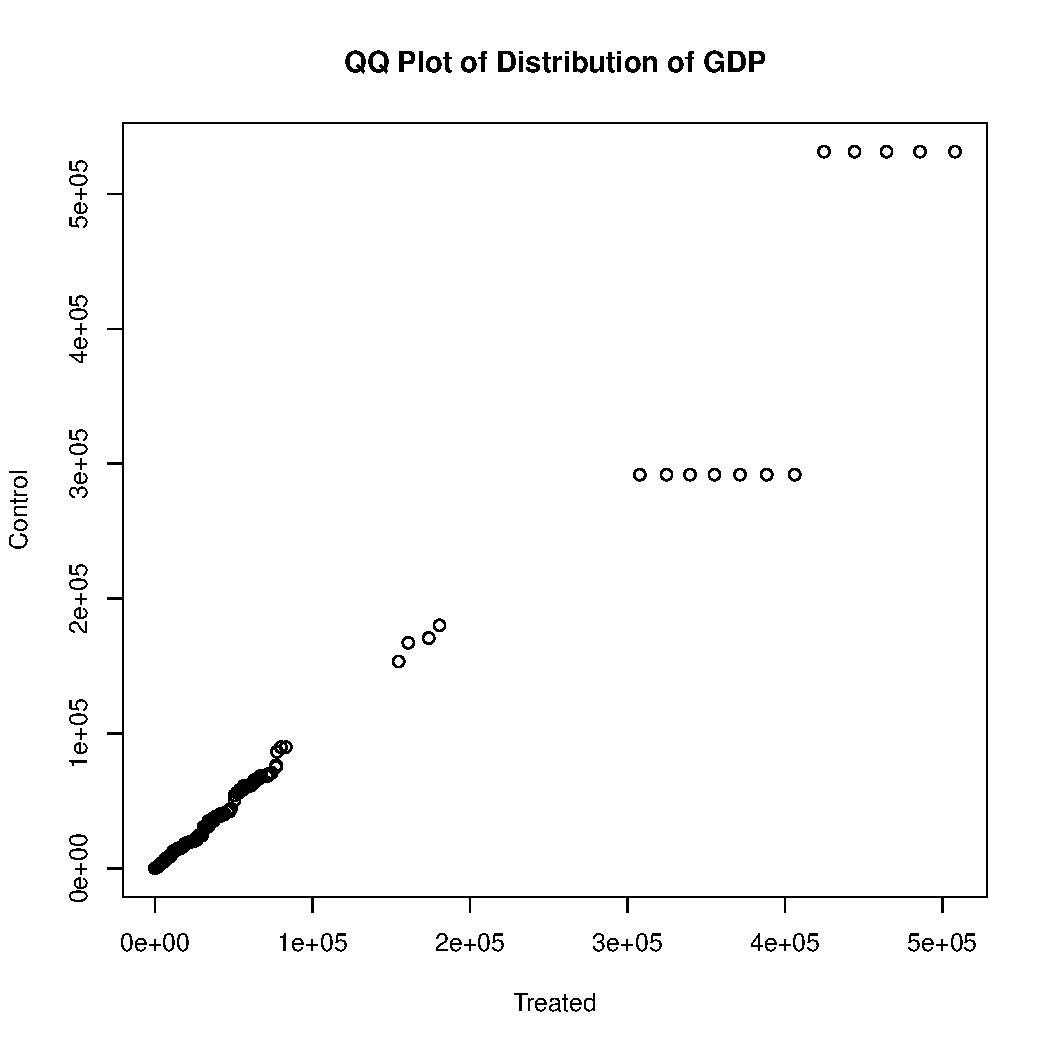
\includegraphics[width=\maxwidth]{figure/unnamed-chunk-3-5} 

\end{knitrout}

\begin{kframe}
\begin{alltt}
\hlkwd{stargazer}\hlstd{(mgen1,} \hlkwc{title} \hlstd{=} \hlstr{"Summary Statistics"}\hlstd{)}
\end{alltt}
\end{kframe}
% Error: Unrecognized object type.


\begin{knitrout}
\definecolor{shadecolor}{rgb}{0.969, 0.969, 0.969}\color{fgcolor}\begin{kframe}
\begin{alltt}
\hlkwd{library}\hlstd{(ggplot2)}
\hlkwd{library}\hlstd{(scales)}
\end{alltt}


{\ttfamily\noindent\itshape\color{messagecolor}{\#\# \\\#\# Attaching package: 'scales'\\\#\# \\\#\# The following objects are masked from 'package:readr':\\\#\# \\\#\#\ \ \ \  col\_factor, col\_numeric}}\begin{alltt}
\hlstd{dp} \hlkwb{<-} \hlstd{df} \hlopt
  \hlkwd{group_by}\hlstd{(Year, polity2)} \hlopt
  \hlkwd{filter}\hlstd{(}\hlopt{!}\hlkwd{is.na}\hlstd{(dpolityb))} \hlopt
  \hlkwd{count}\hlstd{(dpolityb, polity2)} \hlopt
  \hlkwd{group_by}\hlstd{(polity2)} \hlopt
  \hlkwd{mutate}\hlstd{(}\hlkwc{Pdpolity} \hlstd{= n}\hlopt{/}\hlkwd{sum}\hlstd{(n))} \hlopt
  \hlkwd{filter}\hlstd{(dpolityb} \hlopt{==} \hlnum{1}\hlstd{)} \hlopt
  \hlkwd{select}\hlstd{(polity2, Pdpolity)}

\hlkwd{ggplot}\hlstd{(dp,} \hlkwd{aes}\hlstd{(}\hlkwc{x} \hlstd{= polity2,} \hlkwc{y} \hlstd{= Pdpolity))} \hlopt{+}
  \hlkwd{geom_bar}\hlstd{(}\hlkwc{stat}\hlstd{=}\hlstr{"identity"}\hlstd{)} \hlopt{+}
  \hlkwd{xlab}\hlstd{(}\hlstr{"Polity Score"}\hlstd{)} \hlopt{+}
  \hlkwd{ylab}\hlstd{(}\hlstr{"Probability of Change in Polity Score"}\hlstd{)} \hlopt{+}
  \hlkwd{ggtitle}\hlstd{(}\hlstr{"Distribution of Probability of Change in Polity Score"}\hlstd{)} \hlopt{+}
  \hlkwd{scale_y_continuous}\hlstd{(}\hlkwc{labels}\hlstd{=percent)}
\end{alltt}
\end{kframe}
\includegraphics[width=\maxwidth]{figure/unnamed-chunk-4-1} 
\begin{kframe}\begin{alltt}
\hlstd{k1} \hlkwb{<-} \hlkwd{select}\hlstd{(df, polity2, Pdpolity)}
\hlkwd{set.seed}\hlstd{(}\hlnum{2}\hlstd{)}
\hlstd{fit1} \hlkwb{<-} \hlkwd{kmeans}\hlstd{(k1,} \hlnum{5}\hlstd{)}
\hlkwd{aggregate}\hlstd{(k1,}\hlkwc{by}\hlstd{=}\hlkwd{list}\hlstd{(fit1}\hlopt{$}\hlstd{cluster),}\hlkwc{FUN}\hlstd{=mean)} \hlopt
  \hlkwd{arrange}\hlstd{(}\hlopt{-}\hlstd{polity2)}
\end{alltt}
\begin{verbatim}
##   Group.1    polity2   Pdpolity
## 1       3  9.3669951 0.05869939
## 2       1  5.6035714 0.17439929
## 3       4 -0.4593023 0.27545742
## 4       5 -4.9204301 0.21363801
## 5       2 -7.8866758 0.05593759
\end{verbatim}
\begin{alltt}
\hlstd{k1} \hlkwb{<-} \hlkwd{data.frame}\hlstd{(k1, fit1}\hlopt{$}\hlstd{cluster)} \hlopt
  \hlkwd{mutate}\hlstd{(}\hlkwc{fit1.cluster} \hlstd{= plyr}\hlopt{::}\hlkwd{mapvalues}\hlstd{(fit1.cluster,} \hlkwc{from} \hlstd{=} \hlkwd{c}\hlstd{(}\hlnum{3}\hlstd{,} \hlnum{1}\hlstd{,} \hlnum{4}\hlstd{,} \hlnum{5}\hlstd{,} \hlnum{2}\hlstd{),} \hlkwc{to} \hlstd{=} \hlkwd{c}\hlstd{(}\hlnum{1}\hlstd{,} \hlnum{2}\hlstd{,} \hlnum{3}\hlstd{,} \hlnum{4}\hlstd{,} \hlnum{5}\hlstd{)))} \hlopt
    \hlkwd{select}\hlstd{(}\hlkwc{cluster} \hlstd{= fit1.cluster)}

\hlstd{df} \hlkwb{<-} \hlkwd{cbind}\hlstd{(df, k1)}
\end{alltt}
\end{kframe}
\end{knitrout}

\end{document}
